%!TEX root = ../report.tex

\begin{document}
    \chapter{Solution}

   \section{Hand crafted feature extraction}  
   First approach to analyze and explore the domain knowledge of the raw signal from accelerometer is calculating temporal, spectral and statistical aspects of the data. As discussed in chapter 3 domain specific knowledge can be extracted from time-series data to analyze it and used as input to machine learning algorithms as raw signal cannot be used directly. Along with the calculated features we have prior information that has been extracted from the signal that is, penetration and maximum velocity. The dataset contains three signals acceleration, velocity and position that are passed to feature extractor which extracts fixed set of features. Figure \ref{n0} shows example of set of features that have been extracted.
   
   \begin{figure}[h]
   	\centering
   	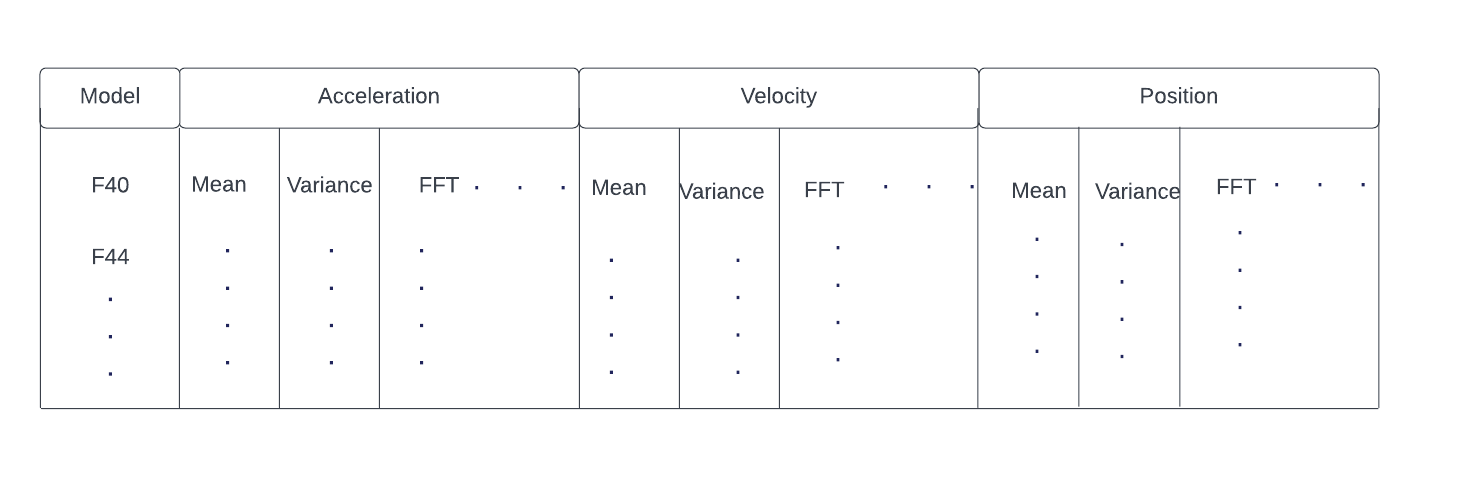
\includegraphics[width=1\linewidth]{images/featable.png}
   	\caption{Handcrafted features }
   	\label{n0}
   \end{figure}
   
   \begin{table}[h]
   	\centering
   	\begin{tabular}{|l|l|}
   		\hline
   		Type    & Features                                                                                                                                                                      \\ \hline
   		Statistical & \begin{tabular}[c]{@{}l@{}}Minimum, Maximum, Median, Mean absolute deviation, \\ Median absolute deviation, \\ Root mean square, Standard deviation, \\ Variance\end{tabular} \\ \hline
   		Temporal    & \begin{tabular}[c]{@{}l@{}}Mean absolute differences, Mean differences, \\ Median differences, Median absolute differences,\\  Entropy\end{tabular}                           \\ \hline
   		Spectral    & \begin{tabular}[c]{@{}l@{}}FFT mean coefficient, Minimum frequency, \\ Maximum frequency, Median frequency, \\ Fundamental frequency\end{tabular}                             \\ \hline
   	\end{tabular}
   	\caption{Fixed set of hand crafted features}
   	\label{t1}
   \end{table}
   
   
   
   The extractor function returns in total 54 features for each car door instance. Table \ref{t1} gives the overview of features calculated for each signal. The dimensionality of the feature vector obtained for each signal is reduced by removing the redundant features and selecting relevant ones by use of Random forest algorithm. This information is passed to supervised machine learning algorithm for classification.
   
   \section{Autoencoder for anomaly detection}   
   To apply a general classification approach there is a requirement of fixed number of classes to separate the data. The problem that is solved by this project contains two classes normal and abnormal. Proper definition of what distinct feature that can classify the signals into these classes is missing. In other words prior information on to what can be called as anomaly is not available because the data we are dealing with is a complex industrial dataset.  Also the data that is provided is highly imbalanced which has been seen during the data analysis in section $4.2.1$. Therefore a direct implementation of deep-learning algorithm to this problem is difficult. These problems arise when we try to find a classification algorithm to solve the problem. To overcome these issues we propose to re frame the problem as anomaly detection using autoencoder.
   
    \begin{figure}[h]
    	\centering
    	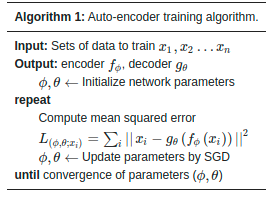
\includegraphics[width=0.5\linewidth]{images/algau.png}
    	\caption{Algorithm for anomaly detection \cite{oh2018residual} }
    	\label{nv0}
    \end{figure}
   
   Detailed discussion on general structure of autoencoder is done in chapter 3 section $3.1.3$. The model is based on low-dimensional latent spaces which have high-level abstract features. Generating models such as interpretation or interpolation are not needed \cite{oh2018residual}. We do not require prior knowledge of latent variables in order to identify anomalies or outliers. Therefore as prior knowledge is not available general autoencoder is suitable for the problem.
   
   The network has same number of inputs and outputs. The goal of this network is to minimize the reconstruction error between the decoded signal and the original. The problem now can be re-framed as regression rather than classification thus mean squared error is suitable for the problem to be solved. 
   
   
   
    \begin{figure}[h]
    	\centering
    	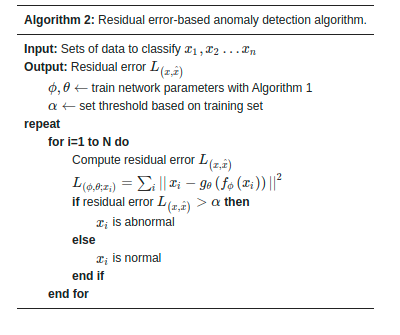
\includegraphics[width=0.75\linewidth]{images/rsd.png}
    	\caption{Algorithm for anomaly detection \cite{oh2018residual} }
    	\label{n00}
    \end{figure}
    
    During compression and expansion, the auto-encoder minimizes the loss of information. Although the decoder restores the high-frequency components to their maximum, the loss of the high-frequency components occurs during the compression process of the encoder. Signals are sampled for each element and reconstructed with the goal of reducing the average difference between input and output signals. The reconstructed signal is not equivalent to the original signal.Instead of focusing on if the input is normal or abnormal the reconstruction error is considered. The algorithm learns higher abstraction of data because of dimension reduction.
    
    In the residual error based anomaly detection algorithm computation of the threshold is done based on the validation set. A optimal threshold can be selected if the it is computed based on abnormal data.
    
  
   \section{Transfer learning with raw signal data}
   

   
   
   \section{Autoencoder as feature extractor}    
   
   
   \section{Transfer learning with spectrogram}   
  There is a significant work done to designing networks to classify and extracting features from spectrogram. Finding a suitable deep-learning model when we have low instances of data is difficult. Therefore transfer learning is helpful solving this problem. Various popular networks architectures such as VGG and Resnet have been used to extract features from spectogram data. For this project VGG is used. 
  
  VGG which is a image classification model and has no relation to the temporal domain knowledge in its design. Also as discussed earlier a clear definition to anomaly is missing. 
  
  
  
  Audio CNNs can be designed considering domain knowledge or not (for further info, see this article). And, without any doubt, spectrogram-based VGGs utilize no audio domain knowledge for their design. What’s good about that?
  By means of not considering any domain knowledge during their design, one minimizes the assumptions the model does w.r.t. the problem. This might be beneficial, for example, if one is not certain in how to approach the task.
  Remember that part of the deep learning game is to allow the architectures to freely discover features, what leads to very successful models. If we specifically design a model to efficiently learn timbral or temporal features, we might inquire the risk of restricting too much the solution space.
  Instead, VGGs are designed to make minimal assumptions over the nature of the signal or problem — so that any structure can be learnt via hierarchically combining small-context representations. Consequently, VGGs inquire the risk of being super-flexible function approximators (as opposed to be regularized models). That’s why people use VGGs, because in some cases this flexibility can be useful! 
\end{document}
